\section{Case Study}
In this section, we first introduce three commonly used scientific workflows that vary from in situ workflow to offline workflow. Then, we evaluate and compare several different workflow launching approaches by trying to adopt the three workflows.

\subsection{Workflows in Case Study}
\subsubsection{VPIC}
Vector Particle-In-Cell (VPIC) is a general purpose particle-in-cell simulation code for modeling kinetic plasmas in multiple spatial dimensions \cite{bowers20080, bowers2008ultrahigh, bowers2009advances}. In our customized VPIC workflow, we perform turbulence simulation using VPIC with in situ analysis using ParaView. ParaView \cite{ahrens2005paraview, ayachit2015paraview} is an open-source, multi-platform data analysis and visualization application. ParaView users can quickly build visualizations to analyze their data using qualitative and quantitative techniques. The ParaView tool in our workflow has two parts: ParaView Server and ParaView Client. ParaView Server runs on the same computing system as the scientific application and is responsible for gathering and rendering visualization data from VPIC. ParaView Client runs on the users' local machines and is responsible for displaying visualized scientific data by connecting with ParaView Server.

In our customized VPIC workflow, we use ParaView Server to perform disk-based in situ analysis, then, via the network, transfer visualized results to the local ParaView Client. The overall workflow is shown in \textbf{Fig. \ref{vpic-workflow}}. The abstracted DAG is represented as \textbf{Fig. \ref{vpic-dag}}.


\begin{figure}
\centering
   \begin{subfigure}[b]{0.4\textwidth}
   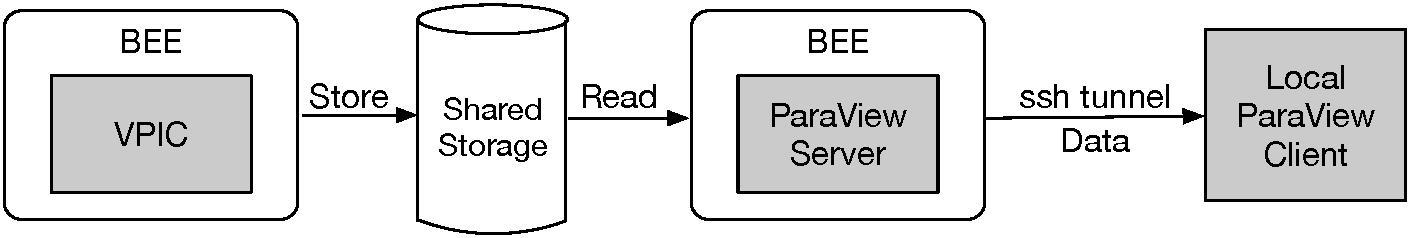
\includegraphics[width=0.9\linewidth]{figures/vpic.pdf}
   \caption{Components and logic in VPIC workflow}
   \label{vpic-workflow} 
\end{subfigure}

\begin{subfigure}[b]{0.4\textwidth}
   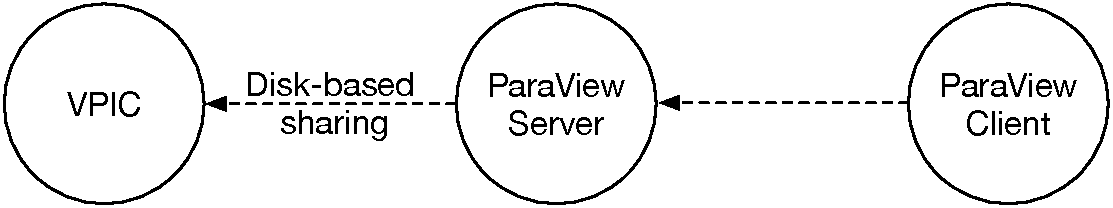
\includegraphics[width=0.9\linewidth]{figures/vpic-dag.pdf}
   \caption{DAG dependency graph in VPIC workflow}
   \label{vpic-dag}
\end{subfigure}
\caption{VPIC workflow}

\end{figure}


\subsubsection{Flecsale}
Flecsale \cite{flecsale} is another workflow similar to the previous VPIC workflow. Flecsale is a computer software package developed for studying problems that can be characterized using continuum dynamics, such as fluid flow. In this workflow, we build Flecsale with Catalyst so that it can enable network-based in situ analysis with simulation control from ParaView. The connection is established using the previously mentioned SSH tunnel. The workflow is shown in \textbf{Fig. \ref{flecsale-workflow}}. We construct the DAG for this Flecsale workflow as in \textbf{Fig. \ref{flecsale-dag}}.

\begin{figure}
\centering
   \begin{subfigure}[b]{0.4\textwidth}
   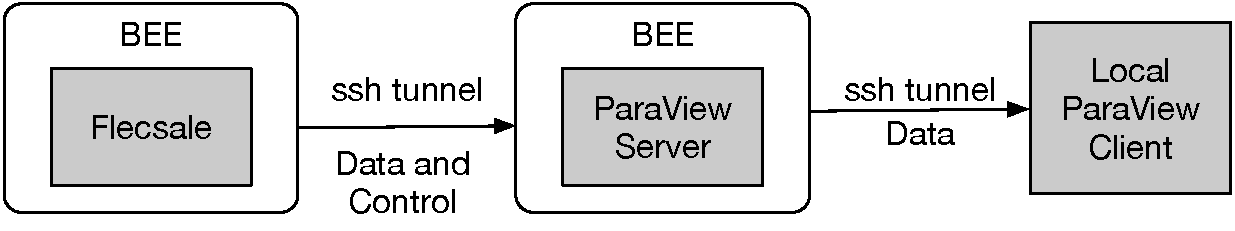
\includegraphics[width=0.9\linewidth]{figures/flecsale.pdf}
   \caption{Components and logic in Flecsale workflow}
   \label{flecsale-workflow} 
\end{subfigure}

\begin{subfigure}[b]{0.4\textwidth}
   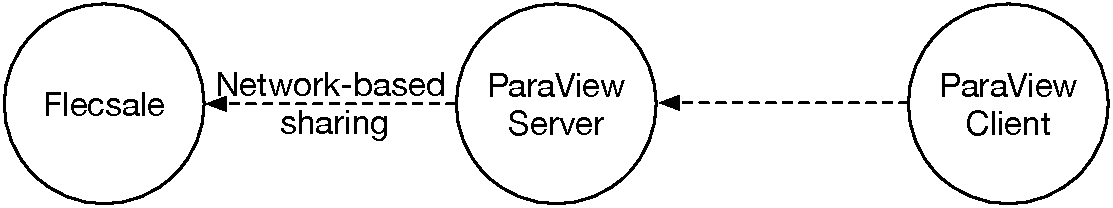
\includegraphics[width=0.9\linewidth]{figures/flecsale-dag.pdf}
   \caption{DAG dependency graph in Flecsale workflow}
   \label{flecsale-dag}
\end{subfigure}
\caption{Flecsale workflow}
\end{figure}

\subsubsection{BLAST}
In our third workflow evaluation, we choose a traditional BLAST workflow for DNA sequence matching. BLAST is a biological application aimed to find similarities between biological sequences \cite{altschul1990basic}. In the BLAST workflow, first a DNA splitter divides the large-sized input DNA sequences into several partitions. Then, it launches several BLAST workers to work on one partition each. Finally, when all workers have done their job, a result collecting worker gathers all the results from each worker and merges them into one output file. The workflow is shown in \textbf{Fig. \ref{blast-workflow}}.
 
The dependencies in this workflow are all offline. The DNA splitter has no depending task, so it can start as soon as we start the workflow. All workers must wait for the splitter, so this is an offline dependency. The result collector needs to wait for all workers, so this is also an offline dependency. All intermediate data are shared through files on disk, so all dependencies are using disk-based sharing. The DAG of this workflow is shown in \textbf{Fig. \ref{blast-dag}}.

\begin{figure}[h]
\centering
   \begin{subfigure}[b]{0.4\textwidth}
   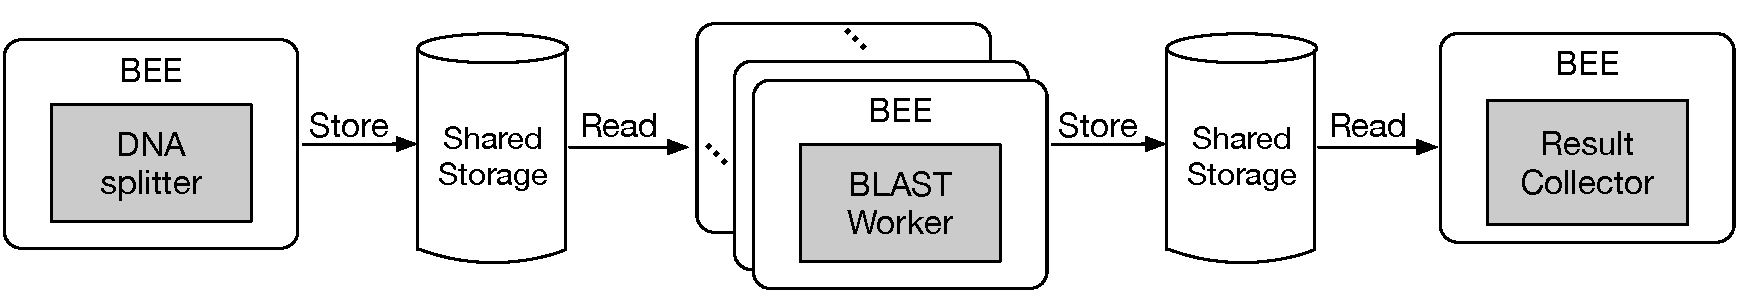
\includegraphics[width=0.9\linewidth]{figures/blast.pdf}
   \caption{Components and logics in BLAST workflow}
   \label{blast-workflow} 
\end{subfigure}

\begin{subfigure}[b]{0.4\textwidth}
   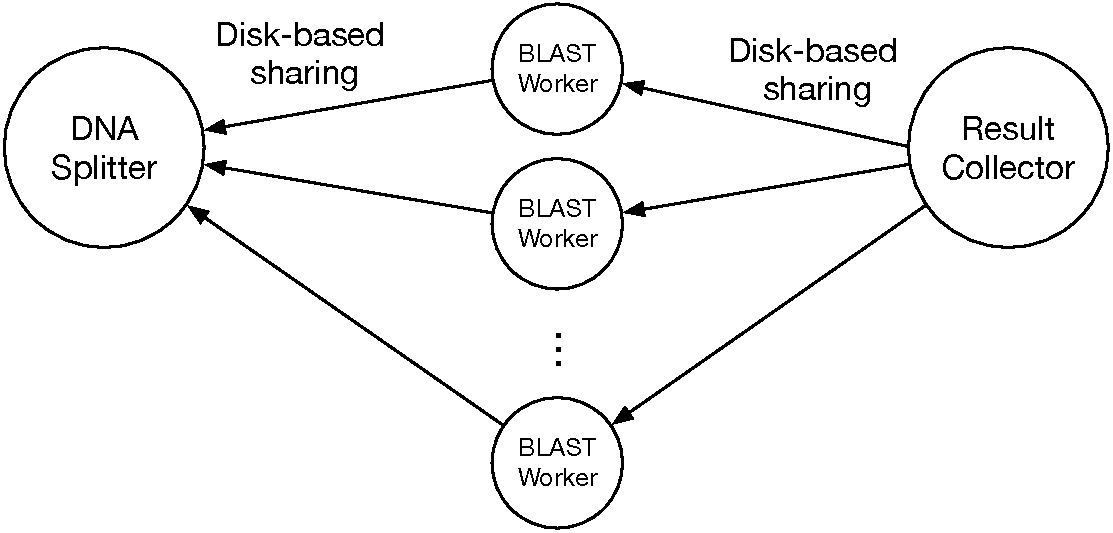
\includegraphics[width=0.9\linewidth]{figures/blast-dag.pdf}
   \caption{DAG dependency graph in BLAST workflow}
   \label{blast-dag}
\end{subfigure}
\caption{BLAST workflow}
\end{figure}



\subsection{Evaluation Methodology}
We evaluate \texttt{BeeFlow} by comparing it with a manual launch approach and another container-based workflow tool -- MakeFlow \cite{albrecht2012makeflow}. The reason we compare \texttt{BeeFlow} with MakeFlow instead of other workflow management tools is that MakeFlow has the most similar functionalities to \texttt{BeeFlow}. We use MakeFlow in the default way as shown in their official use case examples \cite{makeflow-examples}. We also compare to the manual approach, because it is the only method, other than \texttt{BeeFlow}, that we know can launch an in situ workflow. We focus on evaluating three aspects: in situ analysis support, usage complexity, and usage time cost.

The evaluation is conducted on our testbed cluster -- Darwin. It has a `Galton` node partition with KVM enabled. Each node has two 8-core Intel Ivy Bridge E5-2650 v2 processors with 251 GB RAM. For the cloud system, we use Amazon Web Services EC2. The results on AWS are similar to the HPC system results, so we omit results of AWS due to page space limit.

\subsection{Evaluation Results}
\subsubsection{in situ Analysis Support}
We first evaluate the in situ analysis support of different workflow launching approaches. Although MakeFlow is similar to \texttt{BeeFlow}, it does not natively support in situ analysis. It only supports offline dependency as specified in each line of its workflow description files. The manual approach brings the freedom to support any kind of dependencies, including in situ analysis. However, it also costs users considerable time and effort to manually launch each task following each dependency rule. \texttt{BeeFlow} natively supports in situ analysis workflow as well as offline workflow. Its automation feature minimizes the usage complexity and time cost. Both \texttt{BeeFlow} and the manual approach can launch VPIC, Flecsale, and BLAST workflows. MakeFlow, on the other hand, only supports launching the BLAST workflow.


\subsubsection{Usage Complexity}
We then compare the usage complexity of each approach. There are many aspects that affect the usage complexity of an approach. The usage complexity is affected by the total number of command lines that need to be specified by users  and the complexity of constructing/filling configurations files, the total number of configuration sections that need to be configured. So, we define the Usage Complexity as:
\begin{align}
Usage\ Complexity = \nonumber 
Number\ of\ Command\ Lines\ + \\ \nonumber 
Number\ of\ Configuration\ Sections \nonumber 
\end{align}

We evaluate the usage complexity of several main operations:
\begin{itemize}
\item \textbf{Deploying Applications}: Only needed when applications in the workflow are first used or are updated between tests;
\item \textbf{Configuring Workflow}: Only needed when workflow is defined or updated;
\item \textbf{Launching workflow}: Needs to be done for each test.
\end{itemize}

\begin{comment}
\begin{table}[h]
\centering
\caption{Usage Complexity Comparison for Launching VPIC Workflow}
\label{vpic-hpc}
\begin{tabular}{|c|c|c|}
\hline
                       & \texttt{BeeFlow}        & Manual   \\ \hline
Deploying Applications & 6              & 88            \\ \hline
Configuring Workflow  & 2              & 0             \\ \hline
Launching workflow        & 1              & 5             \\ \hline
\end{tabular}
\vspace*{-1em}
\end{table}


\begin{table}[h]
\centering
\caption{Usage Complexity Comparison for Launching Flecsale Workflow}
\label{flecsale-hpc}
\begin{tabular}{|c|c|c|}
\hline
                       & \texttt{BeeFlow}  & Manual      \\ \hline
Deploying Applications & 6              & 86              \\ \hline
Configuring Workflow    & 2              & 0               \\ \hline
Launching workflow        & 1              & 5               \\ \hline
\end{tabular}
\vspace*{-1em}
\end{table}


\begin{table}[]
\centering
\caption{Usage Complexity Comparison for Launching BLAST Workflow}
\label{blast-hpc}
\begin{tabular}{|c|c|c|c|}
\hline
                       & \texttt{BeeFlow}        & Manually                & Makeflow \\ \hline
Deploying Applications & 6                       & 10                      &   10      \\ \hline
Configuring Workflow     & 3                     & 0                       &   m + 2  \\ \hline
Launching workflow        & 1                    & m + 2                   &   1      \\ \hline
\end{tabular}
\vspace*{-1em}
\end{table}
\end{comment}


\begin{table}[]
\centering
\caption{Usage Complexity Comparison for VPIC, Flecsale and BLAST Workflows}
\label{uc}
\begin{tabular}{|c|c|c|c|}
\hline
Approaches             & BeeFlow & Manual & MakeFlow \\ \hline
\multicolumn{4}{|c|}{VPIC Workflow}                  \\ \hline
Deploying Applications & 6       & 88     & N/A      \\ \hline
Configuring Workflow   & 2       & 0      & N/A      \\ \hline
Launching Workflow     & 1       & 5      & N/A      \\ \hline
\multicolumn{4}{|c|}{Flecsale Workflow}              \\ \hline
Deploying Applications & 6       & 86     & N/A      \\ \hline
Configuring Workflow   & 2       & 0      & N/A      \\ \hline
Launching Workflow     & 1       & 5      & N/A      \\ \hline
\multicolumn{4}{|c|}{BLAST Workflow}                 \\ \hline
Deploying Applications & 6       & 10     & 10       \\ \hline
Configuring Workflow   & 3       & 0      & m+2      \\ \hline
Launching Workflow     & 1       & m+2    & 1        \\ \hline
\end{tabular}
\end{table}


We first evaluate the usage complexity of lunching VPIC workflow using \texttt{BeeFlow} and the manual approach. \textbf{Table \ref{uc}} shows the usage complexity for launching the VPIC workflow on Darwin. For deploying applications, among the three applications, only VPIC and ParaView Server need to be configured. \texttt{BeeFlow} uses Docker for deployment, so it only needs a few simple configurations in its job description files. The manual approach, on the other hand, requires users to build and configure applications from scratch, which introduces extra complication and efforts. On Darwin, it requires 60 commands to deploy ParaView Server and 28 commands to deploy VPIC. For configuring workflows, \texttt{BeeFlow} requires two commands for configuring its workflow description files. The manual approach does not need any workflow configuration. Finally, to launch the workflow, only one command is necessary for \texttt{BeeFlow}. Five commands are needed to launch manually. 

Second, we compare the usage complexity of launching the Flecsale workflow using \texttt{BeeFlow} and the manual approach. As shown in \textbf{Table \ref{uc}}, similar to VPIC workflow, \texttt{BeeFlow} has much lower usage complexity than the manual approach for deploying applications with little extra workflow configurations.

Third, we compare the usage complexity of launching BLAST workflow using different approaches. Depending on the user's configuration on the number of workers in this workflow, the total number of tasks varies. \textbf{Table \ref{uc}} shows the usage complexity to launch BLAST workflow on Darwin, in which $m$ represents the number of workers. For deploying the application, Docker-based \texttt{BeeFlow} has lower usage complexity than the manual approach and MakeFlow since they both need manual application deployment. The manual approach does not need workflow configuration, while MakeFlow needs $m+2$ configuration lines (one for each task). \texttt{BeeFlow}, on the other hand, features automation that only needs one configuration for $m$ worker, so it only needs three total configurations. Finally, due to lack of automation, the manual approach has the highest usage complexity when launching the workflow.


\subsubsection{Usage Time Cost}

In this section, we evaluate the time cost of launching each workflow using each approach. The timing results are shown in \textbf{Table \ref{tc}}. We time the deployment of each task in the three workflows on Darwin and the time cost for users to launch each workflow, including wait time due to task dependencies.  The results show, due to the Docker container support, \texttt{BeeFlow} has the shortest application deployment time. This is especially beneficial if target applications require complex and time consuming configurations. For example, the ParaView tool, used by both VPIC and Flecsale workflows, requires at least 30 minutes to build and takes even longer when configured with more features enabled. On the other hand, \texttt{BeeFlow} only needs several minutes to pull Docker images. Although MakeFlow also supports Docker containers, the Docker daemon is usually not supported in current production HPC software stacks, including our testbed Darwin. So, we still need to manually deploy each application when using MakeFlow. 

To launch each workflow, both \texttt{BeeFlow} and MakeFlow feature automation, so only several seconds are needed to initialize workflow tools and launch each workflow (users do not need to wait). For the manual approach, users need to wait for each task to become ready, and then launch the next task. For example, in the VPIC workflow, users need to first start the VPIC simulation manually, then wait for 34 seconds before they can launch ParaView for in situ analysis. The lack of automation can cost users extra time.


\begin{comment}
\begin{table}[]
\centering
\caption{Time cost of VPIC workflow}
\label{vpic-time}
\begin{tabular}{|l|l|l|}
\hline
                        & \texttt{BeeFlow} & Manual \\ \hline
Application deployment  & 2m25s            & 78m31s \\ \hline    
Launch workflow         & 3s               & 34s    \\ \hline
\end{tabular}
\vspace*{-1em}
\end{table}

\begin{table}[]
\centering
\caption{Time cost of Flecsale workflow}
\label{flecsale-time}
\begin{tabular}{|l|l|l|}
\hline
                        & \texttt{BeeFlow} & Manual  \\ \hline
Application deployment  & 2m5s             & 36m20s  \\ \hline    
Launch workflow         & 3s               & 1m5s    \\ \hline
\end{tabular}
\vspace*{-1em}
\end{table}

\begin{table}[]
\vspace*{-1em}
\centering
\caption{Time cost of BLAST workflow}
\label{blast-time}
\begin{tabular}{|l|l|l|l|}
\hline
                        & \texttt{BeeFlow} & Manual  & MakeFlow \\ \hline
Application deployment  & 40s              & 2m22s   & 2m22s    \\ \hline    
Launch workflow         & 3s               & 4m44s   & 3s       \\ \hline
\end{tabular}
\vspace*{-1em}
\end{table}

\end{comment}

\begin{table}[]
\centering
\caption{Time cost of launching VPIC, Flecsale and BLAST Workflows}
\label{tc}
\begin{tabular}{|c|c|c|c|}
\hline
Approaches             & BeeFlow & Manual & MakeFlow \\ \hline
\multicolumn{4}{|c|}{VPIC Workflow}                  \\ \hline
Deploying Applications & 2m25s   & 78m31s & N/A      \\ \hline
Launching Workflow     & 3s      & 34s    & N/A      \\ \hline
\multicolumn{4}{|c|}{Flecsale Workflow}              \\ \hline
Deploying Applications & 2m5s    & 36m20s & N/A      \\ \hline
Launching Workflow     & 3s      & 1m5s   & N/A      \\ \hline
\multicolumn{4}{|c|}{BLAST Workflow (two workers)}                 \\ \hline
Deploying Applications & 40s     & 2m22s  & 2m22s    \\ \hline
Launching Workflow     & 3s      & 4m44s  & 3s       \\ \hline
\end{tabular}

\end{table}



